\documentclass[11pt,letterpaper, twocolumn]{article}
\usepackage{graphicx} % Required for inserting images
\usepackage[latin1]{inputenc}
\usepackage{fullpage}
\usepackage{amsmath}
\usepackage{amssymb}
\usepackage{setspace}
\usepackage{hyperref}
\usepackage{float}
\usepackage{fancyhdr}
%multi-row
\usepackage{multirow}
\usepackage[left=0.8in, right=0.8in, top=1in, bottom=1in, headsep=0pt
  ]{geometry}
\title{{\bf Image Processing and Classification Model for Screening Mammography in Automated Detection of Breast Cancer}}
\author{Vinayak Bassi, Youngmin Kim, Chalida Naiyaporn, Nawat Swatthong, Seonho Woo \\
vbassi, yngmkim, chalida, nawatsw, clairewo @umich.edu}
\date{}
\lhead{EECS545}
\rhead{Final Report}
\begin{document}

\maketitle
%%%%%%%%%%%%%%%%%%%%%%%%%%%%%%%%%%%%%%%%%%%%%%%%%%%%%%%%%%%%%%%%%%%%%%%%%%%%%%
\section{Abstract}
% Breast cancer is well-known that it is hardly diagnosed at its early stage. Using image classification to identify its malignancy using machine learning methods will bring up a substantial effect on medical systems and the causality rate of patients. In this analysis, we applied the CNN (Convolutional Neural Network) and ViT (Visual Transformer) models, mostly CNN, to detect breast cancer from mammogram images and evaluate the model performances based on the preprocessing methods and steps. 

% Our preliminary results show that both models without data preprocessing perform poorly and are overfitting. In our next step of model development, data preprocessing will be integrated into the pipeline model and simultaneously combined with other types of cancer X-ray images into the original dataset to improve the classification performance of both ViT and CNN models.

Breast cancer is well-known that it is hardly diagnosed at its early stage, using image classification to identify its malignancy using machine learning methods will bring up a substantial effect on medical systems and the causality rate of patients. In this analysis, we applied the CNN (Convolutional Neural Network) and ViT (Visual Transformer) models, mostly CNN, to detect breast cancer from mammogram images and evaluate the model performances based on the preprocessing methods and steps. 

Since our preliminary results show that baseline models in both architectures without data preprocessing perform poorly, we investigated the best classification model by various combinations of adding image data preprocessing methods. According to experiments with 5-fold cross-validation, we found that the most composite setting with ROI cropping, thresholding, augmentation, and auxiliary variables predictions performs best in CNN (ResNeXt) architecture. In most experiments, we found that the imbalanced nature of the input data significantly affected the model performance in downgrading, especially in the baseline model and implementation of the test data. In the future, we would work on improving model robustness and performance by training ROI extraction on other mammography data and aggregating some ROI crop modules for better ROI crop patches.

\section{Introduction}
Breast cancer has long been recognized as a difficult disease to diagnose in its early stages. The World Health Organization has emphasized the importance of early detection, as cancer cells spread quickly, and the fatality rate increases dramatically as the disease progresses. Mammogram images are currently analyzed by highly-trained radiology experts to distinguish cancerous from non-cancerous tissue. However, the shortage of trained radiologists in many countries has created a pressing need for innovative solutions.

Machine learning techniques offer a promising approach to improving breast cancer detection in mammography. By supplementing the skills of human radiologists, these tools could help detect the disease in its earliest stages. This technology has the potential to improve patient outcomes while also increasing the efficiency of the healthcare system. By freeing up medical professionals' time and reducing costs, automated detection systems could enable healthcare providers to focus on other essential tasks and improve patient care. Overall, implementing machine learning techniques for breast cancer detection represents a promising opportunity to impact healthcare outcomes positively.

%%%%%%%%%%%%%%%%%%%%%%%%%%%%%%%%%%%%%%%%%%%%%%%%%%%%%%%%%%%%%%%%%%%%%%%%%%%%%%%%%%%%%%%%%%%%
\section{Related Works}
With the advent of machine learning and deep learning algorithms, diagnosing cancerous tumors and further treating them has become more efficient. We found research that has used Support Vector Machines (SVM) (Wang et al., 2018; Vijayarajeswari et al., 2019)${}^{[1][2]}$,  Naive Bayes Classifiers(Karabatak, 2015)${}^{[3]}$, and advanced deep learning algorithms (Convolutional Neural Networks, Vision Transformer) (Refat Khan et al.; Chen et al., 2022)${}^{[4][5]}$ to classify and detect breast cancer.
A balanced image dataset in terms of medical images has almost equal representations of both normal and abnormal cases. Much previous research that used neural network frameworks has used a balanced image dataset to classify benign and malignant mammography images. The article by Ragab Dina A. et al.${}^{[6]}$, which uses a deep convolutional neural network and SVM to classify breast cancer mammography images, has reported the use of the Curated Breast Imaging Subset of DDSM (CBIS-DDSM) which is a balanced dataset.

Generally, the available dataset for image mammograms is an imbalanced dataset. Imbalance datasets pose a significant challenge for developing deep learning models, especially CNN. We saw in some research work where they have used pre-trained CNN on a sample of DDSM database (an unbalanced mammograms dataset) (Tsochatzidis L. et al.)${}^{[7]}$. To address the issue of imbalance, researchers have explored various techniques, such as oversampling, undersampling, and data augmentation, to balance the datasets and improve the performance of CNNs. Additionally, transfer learning, where pre-trained CNNs on large datasets are fine-tuned for breast cancer detection, has also been used to address the imbalance in the datasets.

Our study used an imbalanced dataset provided by the Radiological Society of North America (RSNA) as part of a Kaggle competition. While referencing other submissions in the competition, we saw a strong emphasis on using medical preprocessing techniques such as ROI (Region-of-Interest) cropping and data augmentation techniques. In terms of deep learning models, many have reported the use of pre-trained CNN models fine-tuned for mammograms dataset. The winner of the competition has trained the YOLOx framework on external breast mammograms to generate an enhanced ROI crop and further train those images on a CNN architecture (4 x Convnextv1-small 2048x1024)${}^{[8]}$.

In our study, we have used importance sampling to manage the imbalanced dataset. We also deep-dived into techniques of data augmentation, thresholding, and auxiliary prediction. We have tried to learn cross-entropy auxiliary targets, which include image and auxiliary components (density, implant, BIRADS, etc.) while training which enhanced our prediction score. We also trained the RSNA dataset for a pre-trained ViT model.

%%%%%%%%%%%%%%%%%%%%%%%%%%%%%%%%%%%%%%%%%%%%%%%%%%%%%%%%%%%%%%%%%%%%%%%%%%%%%%%%%%%%%%%%%%%%
\section{Data}
%Description of Imbalanced Data
We use a dataset from the Kaggle competition, which originated from the Radiological Society of North America (RSNA), a non-profit organization that serves as a representative of 31 subspecialties related to radiology from 145 countries globally. The fact regarding 2\% of images contains cancer is both challenging and reflective of real-world situations where only a small number of people have cancer. 

\begin{figure}[H]
    \centering
    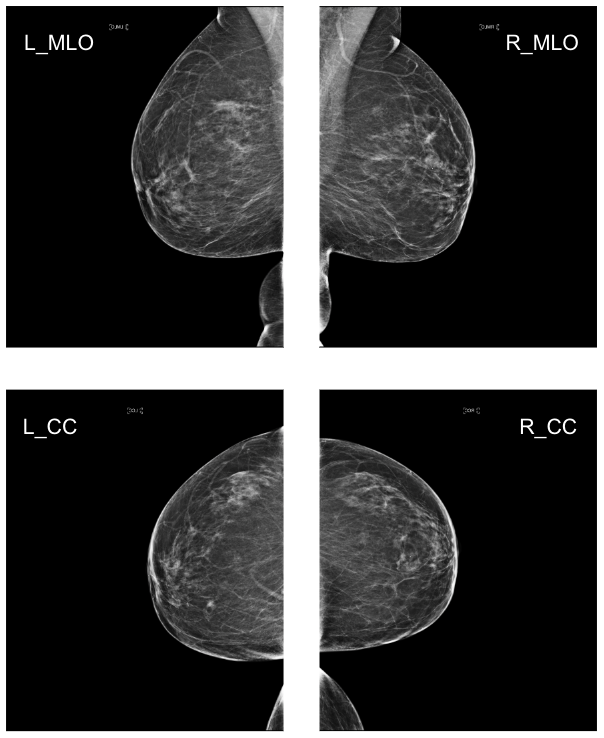
\includegraphics[scale = 0.6]{Final/Figures/L_malignant+R_benign.png}
    \caption{Malignant (left) and Benign (right) Mammograph Sample}
    \label{fig:malignant}
\end{figure}
As shown in Figure 1, it is hardly capable for humans to discriminate between malignant(left) and benign(right) scans.

\begin{figure*}[t]
    \centering
    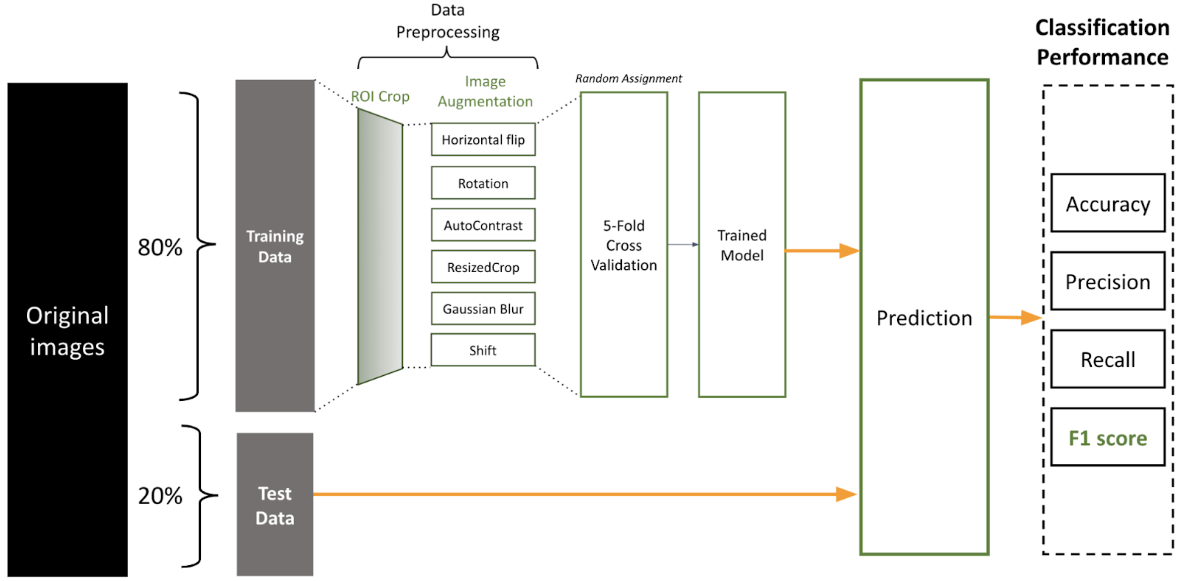
\includegraphics[scale = 0.7]{Final/Figures/model diagram.png}
    \caption{Model Diagram}
    \label{fig:final_model_diagram}
\end{figure*}
The data for mammography breast images were collected from 11,913 patients. Each patient provided 2-side of the breast and at least two views of the orientation: the total number of images in this dataset was 54,706. Apart from the images, there are 9 variables that were collected from patients; age, whether the image was left or right (laterality), the orientation of the image (view: CC, MLO), whether the patient has breast implant (implant), a rating for density of breast tissue (density: A, B, C, D), whether the patient follow-up biopsy (biopsy), whether cancer proved to be an invasive (invasive), diagnosis for breast (BIRDAS: 0-the breast required follow-up, 1-the breast was rated as negative for cancer, and 2-the breast was rated as normal), and whether the case was unusual difficult (difficult\_negative\_case). For analysis, we make image data into training and test groups, split with a 4:1 ratio. 

\begin{table}[H]
\resizebox{\columnwidth}{!}{
\begin{tabular}{|c||c|c|c|}
    \hline
    Images\slash Datasets & Full & Training & Test \\ 
    \hline
    All & 54,760 & 43,805 & 10,901 \\
    Malignant (Cancer) & 1,158 & 917 & 231\\
    Benign (Non-cancer) & 53,548 & 42,878 & 10,670\\
    \hline
\end{tabular}}
\caption{Data sizes per groups}
\end{table}


\subsection{Features}
Since the total number of images was 54,706,  1,158 (2.12\%) images were cancer images. We can see that the images between cancer and non-cancer are imbalanced and might cause a problem in our analysis. So, we decided to deal with the imbalanced data by using the F1 score to evaluate the best model.
\begin{table}[h]
\resizebox{\columnwidth}{!}{
% \footnotesize
\begin{tabular}{|c||c|}
    \hline
    Variables & Median(IQR)\slash \% \\ 
    \hline
    Age & 59 (51, 66) \\ Laterality: Right & 50.16\% \\
    View: MLO & 51.01\% \\ Implant: No & 97.30\% \\
    Density: B & 23.13\% \\ Biopsy & 94.57\% \\
    Invasive & 98.50\% \\ Difficult Negative Case: No & 85.92\% \\
    BIRADS: required follow-up & 15.08\% \\ BIRADS: labeled as negative (Benign) & 28.83\% \\
    BIRADS: labeled as normal & 4.14\% \\ Cancer & 97.88\%\\
    \hline
\end{tabular}}
\caption{Median and Interquartile of features}
\end{table}

Table 2 above shows the median value for each variable in the data with its interquartile range (25\%, 75\%) for the numerical variable or the percent of data for the categorical variables.

%%%%%%%%%%%%%%%%%%%%%%%%%%%%%%%%%%%%%%%%%%%%%%%%%%%%%%%%%%%%%%%%%%%%%%%%%%%%%%%%%%%%%%%%%%%%
\section{Methods}
\begin{figure*}[t]
    \centering
    % 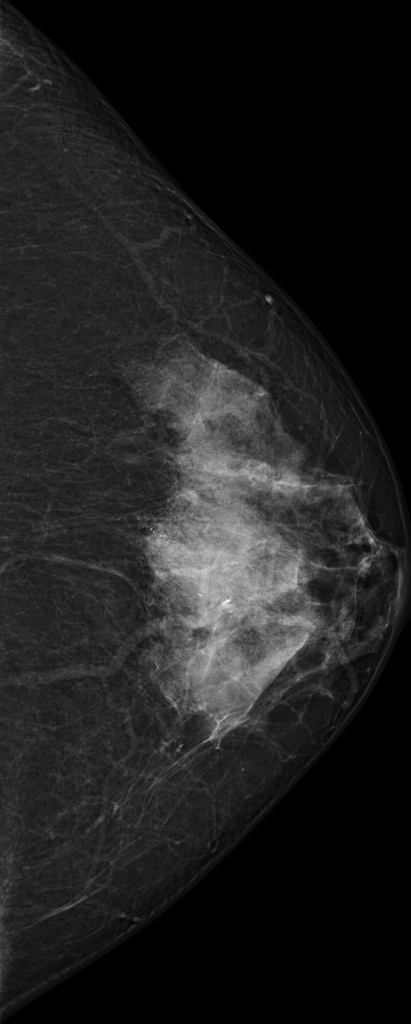
\includegraphics[scale = 0.4]{Final/Figures/Correctly_classify.png}
    % \caption{Well-Predicted Image Sample in classification}
    % \label{fig: classified_True}
    % 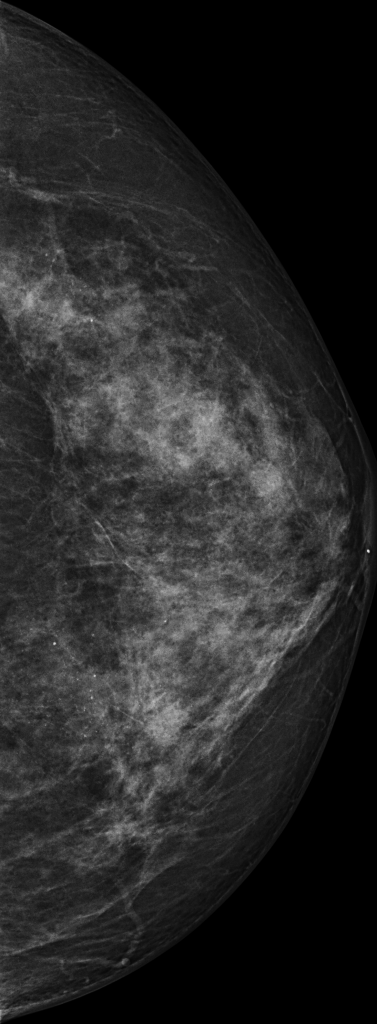
\includegraphics[scale = 0.4]{Final/Figures/Incorrectly_classify.png}
    % \caption{Poorly-Predicted Image Sample in classification}
    % \label{fig: classified_False}
    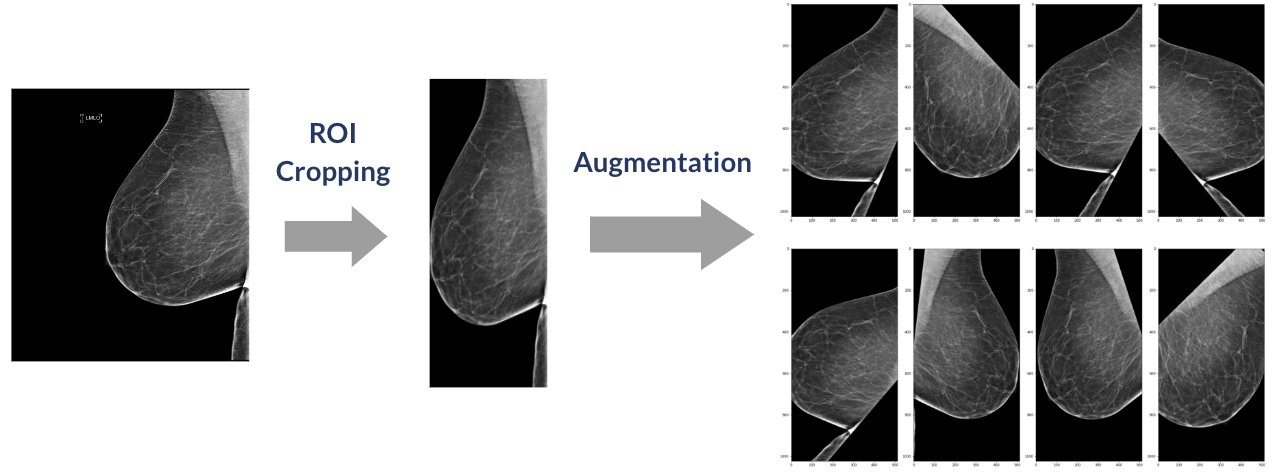
\includegraphics[scale = 0.7]{Final/Figures/image_preprocess.png}
    \caption{ROI Cropped and Augmented Image Sample}
\end{figure*}

This section presents our model architecture, comprising six key components: ROI Crop, Image Augmentation, Backbone ML model, Weighted Loss, Threshold, and Auxiliary Prediction. As depicted in Figure 2 model flow-diagram, our preprocessing pipeline initially employs ROI Crop and Augmentation techniques to enhance each breast cancer image before feeding it into the Backbone model. We experimented with both CNN and ViT pre-trained models as our Backbone model. However, we encountered a challenge in finding a suitable CNN and ViT pre-trained model on medical images. Therefore, we resorted to using general pre-trained CNN and ViT models (on ImageNet) as done by most other researchers in the field${}^{[5][6]}$. 

To address the issue of data imbalance during the training of our ML model, we employed a weighted loss function. To determine the best threshold for distinguishing cancer images, we used a 5-fold cross-validation approach. Finally, we evaluated our model's performance using test data.

\subsection{ROI Cropping}
% \begin{figure}[H]
%     \centering
%     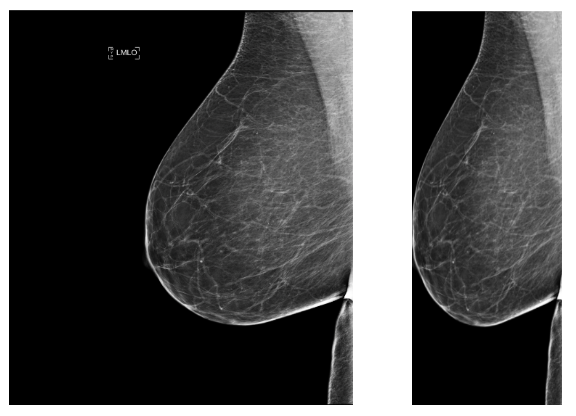
\includegraphics[scale = 0.6]{Final/Figures/original+roi_cropped.png}
%     \caption{Original Image (left) and ROI Cropped Image (right)}
%     \label{fig:sample img for roi crop}
% \end{figure}
ROI(Region of Interest) cropping is a computer vision technique that extracts an image's specific object or area of interest by defining a rectangular region and cropping and resizing the image to include only the relevant pixels. This method is particularly useful when the object is small relative to the overall image or when background noise or clutter can interfere with detection. In our analysis, we employed ROI cropping to extract the breast area and exclude other non-breast regions from the images.

\subsection{Augmentation}
After ROI cropping, we performed image augmentation to increase the diversity and robustness of the dataset by applying multiple transformations. Image augmentation is a computer vision technique that artificially expands the dataset by applying various transformations to the original images. Our analysis employed several transformations, including horizontal flip, rotation, auto contrast, resize crop, Gaussian blur, and shift to increase diversity. Additionally, we reduced noise and improved the model's resilience to small variations in input data by using Gaussian blur. Furthermore, we utilized auto contrast to enhance image contrast, highlighting more details and facilitating cancer detection.
% \begin{figure}[H]
%     \centering
%     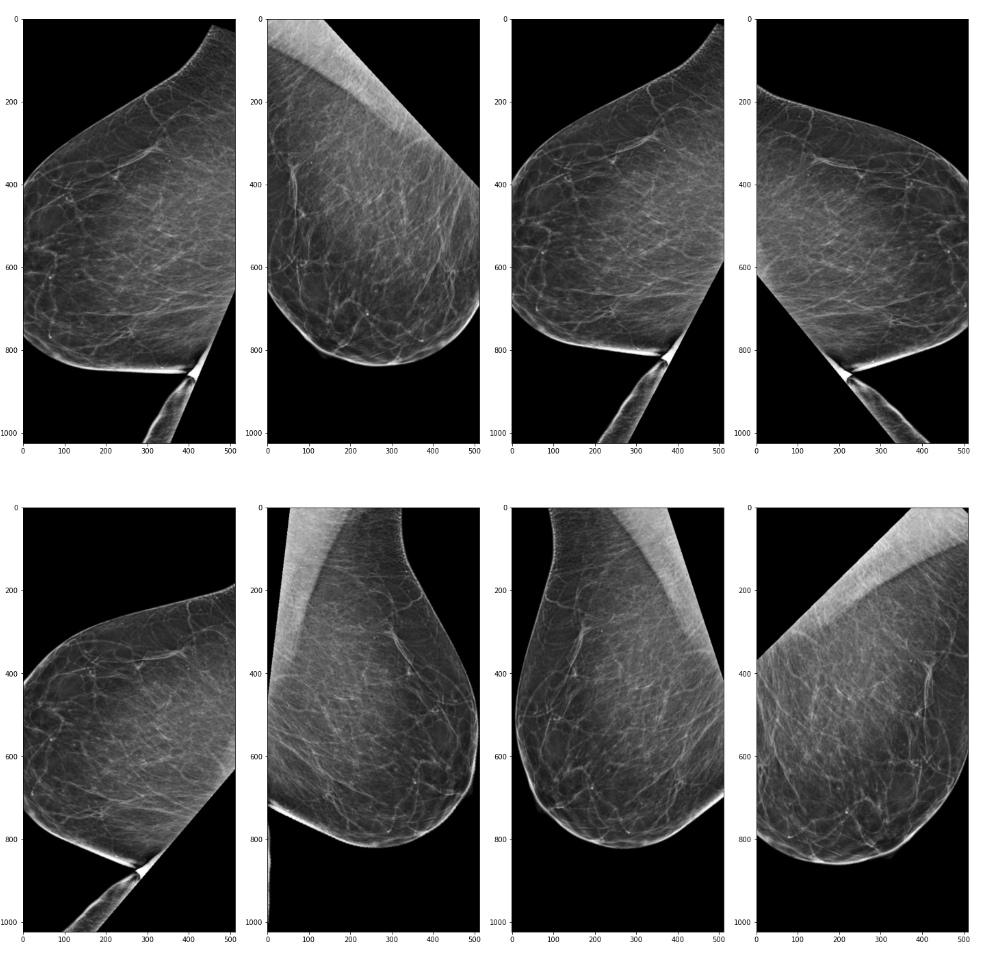
\includegraphics[scale = 0.4]{Final/Figures/augmented.png}
%     \caption{Augmented Image Sample after ROI cropping}
%     \label{fig: sample img for aug}
% \end{figure}

\subsection{Backbone Model}
For our study, we focused majorly on CNN models. We found much research that reported usage of ResNet (Residual Networks) CNN architecture and it's variants. It is a popular CNN architecture that introduced the concept of residual learning to address the vanishing gradient problem in deep networks. It utilizes skip connections to allow the gradients to flow directly through the network, enabling the training of very deep networks. Furthermore, a ResNeXt is a convolutional neural network architecture that builds on the ResNet architecture by introducing a new 'cardinality' element.  It repeats a building block that aggregates a set of transformations with the same topology, thus capturing more diverse features. We saw our best results using a variant of ResNext, called SE ResNeXt. 

Furthermore, we also used state-of-the-art architecture in the form of a Vision Transformer (ViT). By replacing conventional convolutional layers with self-attention layers, a Vit architecture is reported to enable the network to process image patches in a more flexible and efficient manner. For our study, we used pre-trained models in the family of DeiT family of ViT models. The base architecture consists of a stack of transformer blocks, with each block having self-attention and feedforward layers.

\subsubsection{Weighted Loss}
As we explained in the \textit{Section 4: Data}, we choose a highly imbalanced dataset that is more likely to be found in reality. To solve this imbalance, we use the weighted loss function, one of the most well-known techniques to tackle a problem in imbalanced data, giving more weight to the loss of cancer images. We employed weighted loss rather than weighted sampling since it performed better empirically.

\subsubsection{Threshold}
For setting the threshold, we used the sigmoid function since there are only two classes in the dataset (malignant and benign) in order to improve the model performance by discriminating between malignant (cancer) and benign (non-cancer) images in evaluation and testing. The best threshold was determined by evaluation data and results, and then it was employed in the testing set.
 
\subsubsection{Auxiliary Prediction}
In addition to the techniques described in Sections 4.4 and 4.5, we have incorporated auxiliary loss predictions into our model by adding extra output branches to the network that predict intermediate outcomes related to the main task of classifying mammogram images. Our approach uses 11 additional features (listed in Table 2) as intermediate predictions to compute additional loss, which is then combined with the main loss function to optimize the model during training. Incorporating auxiliary loss predictions has been shown to help improve model performance by reducing the risk of gradient vanishing, promoting the learning of diverse features, preventing overfitting, and providing regularization to the network. ${}^{[9]}$

\subsection{Experiment}
In this section, we explain our experiment settings and evaluation metrics. Also, we illustrate our baseline and follow-up models in which our major components are added to a baseline model.

\subsection{Experiment Settings and Evaluation Metrics} 
We utilize 5-fold cross-validation to evaluate all models with our training dataset. Original images are high-resolution dcm(dicom) format files, so we converted dcm files to png files. Also, to reduce the training and test overhead and fit a pre-trained backbone model, we resized images to smaller sizes. About the model parameters, first, we adopt other competitors’ parameters and change them little by little to get a better result. We finetune our model for 3-10 epochs(depending on the backbone model). The batch size is 16, and the learning rate is 0.0002 to 0.0008. For backbone models we tried both freezing(transfer learning) and no freezing, but all models we tested made better results without freezing.

\subsection{Baseline and Implemented Model Description}
% We set our baseline is just applying a backbone model on resized original images (none of ROI crop, augmentation or others) with weighted loss. We tested two backbone models. One is CNN named 'seresnext50\_32x4d' and the other is ViT named 'deit3\_base\_patch16\_384'. We tried other models such as eva02, swin-ViT, google/vit, but the above models made better performance. After we found out CNN makes better results on average, we added components one by one to our backbone model. Also, most kaggle participants and almost all top rankers use CNN.

% First, we added an ROI crop to get more useful images. Original images have large useless black pixel area, so we found ROI cropped images from kaggle site and used it. This is our second model.

% Next, we added threshold technique. We realized that if we use threshold values which discriminate against cancer images other than 0.5, validation f1 score improves. Also, sometimes(not always) it also lead to better test result, too. We calculate the f1 score varying threshold value from 0 to 1 by 0.01, and choose the best threshold value that makes the best f1 score of that CV fold. We choose the best fold model with threshold value and apply it to test data. This is our third model.

% Third, we add image augmentation components. Because all images are ROI cropped x-ray images of breasts, we assume that a big change in image is not useful. Therefore, we apply little changes such as rotate a little, resize a little bit and crop. This is our fourth model.

% Finally, we adopt Auxiliary Prediction. Before adding this component, our model only predicts cancer or not and also loss is only dependent on cancer because our goal is predicting cancer images. However, our model predicts other features in kaggle data. There are 11 features that can predict which is 'site\_id', 'laterality', 'view', 'implant', 'biopsy', 'invasive', 'BIRADS', 'density', 'difficult\_negative\_case', 'machine\_id', 'age'. Our model predicts these 11 features and calculates loss. This loss is also used during backpropagation. This is our fifth and final model.

For the baseline model, we applied only a backbone model on resized original images with a weighted loss function. Specifically, we employed two backbone models, the 'seresnext50\_32x4d' CNN and the 'deit3\_base\_patch16\_384' ViT. While we evaluated several other models, including eva02, swin-ViT, and google/vit, our chosen backbone models demonstrated superior performance. Given that CNN models were prevalent among top Kaggle participants, we opted to focus on this type of model. 

To improve performance, we gradually introduced several additional components to our baseline model. Firstly, we incorporated an ROI crop module to eliminate useless black pixel areas in the original images. We obtained ROI-cropped images from Kaggle's public dataset and applied them as the basis for our second model. 

Secondly, we introduced thresholding techniques to identify cancer images with improved accuracy. By varying the threshold value from 0 to 1 in increments of 0.01, we computed the F1 score and selected the best threshold value that resulted in the highest F1 score. We applied this approach to both validation and test datasets, resulting in our third model. 
%%%%%%%%%%%%%%%%%%%%%%%%%%%%%%%%%%%%%%%%%%%%%%%%%%%%%%%%%%%%%%%%%%
%%%%% RESULT TABLE %%%%%
\begin{table*}[t]
\centering
%\resizebox{\columnwidth}{!}{
%\footnotesize
\begin{tabular}{|c|c|c|c|c|c|c|}
    \hline
\multicolumn{2}{|c|}{ } & Evaluation &  \multicolumn{4}{c|}{Test} \\
\hline
Setting & Model & F1 & F1 & Recall & Precision & Accuracy \\
\hline\hline
\multirow{2}{*}{Resized Original} & CNN(ResNeXt) & 0.047 & 0.027 & 0.022 & 0.035 & 0.966 \\
& ViT(deit3) & 0.037 & 0.0 & 0.0 & 0.0 & 0.979 \\
\hline
+ ROI Crop & CNN & 0.057 & 0.108 & 0.359 & 0.063 & 0.874\\
\hline
+ Threshold & CNN & 0.122 & 0.076 & 0.351 & 0.043 & 0.820 \\
\hline
+ Augmentation & CNN & 0.161 & 0.044 & 0.043 & 0.043 & 0.959\\
\hline
\multirow{2}{*}{+ Auxiliary Prediction} & CNN(ResNeXt) & 0.345 &  0.314 & 0.290 & 0.342 & 0.973 \\
& ViT(deit3) & 0.130 & 0.063 & 0.126 & 0.042 & 0.921 \\
\hline
\end{tabular}%}
\caption{Results of Models Implementation}
\end{table*}
%%%%%%%%%%%%%%%%%%%%%%%%%%%%%%%%%%%%%%%%%%%%%%%%%%%%%%%%%%%%%%%%%%
Next, we introduced image augmentation to the ROI-cropped X-ray images of breasts. As we assumed that large image changes were not useful, we applied minor alterations such as slight rotation, resizing, and cropping. This resulted in our fourth model. 

Finally, we incorporated an auxiliary prediction module to predict features beyond cancer/non-cancer. Specifically, we trained our model to predict 11 additional features, including site\_id, laterality, view, implant, biopsy, invasive, BIRADS, density, difficult\_negative\_case, machine\_id, and age. This module enabled our model to capture more information and improve overall performance.


%%%%%%%%%%%%%%%%%%%%%%%%%%%%%%%%%%%%%%%%%%%%%%%%%%%%%%%%%%%%%%%%%%%%%%%%%%%%%%%%%%%%%%%%%%%%

\section{Result and Discussion}
In our study, we initially compared the performance of Convolutional Neural Network (CNN) and Visual Transformer (ViT) models for predicting breast cancer using mammography images. However, after testing several ViT models, we found that they did not perform well, which led us to focus on CNN models for our experiments. As shown in Table 3, we tested several methods to address the imbalance, and it turned out to have an actual improvement in model performance. 

The baseline model using the original image with only resizing demonstrates a poor performance of F1 score below 0.05 for both models in the evaluation set, which is probably due to imbalanced data.  However, as we add each step of ROI cropping, Threshold, Augmentation, and Auxiliary, gradual improvement in their performance is observed. We used 5-fold cross-validation in training data to determine the best classification model with multiple composite data preprocessing techniques tested in this experiment. 

In contrast to better performance in most composite model settings using evaluation data, as expected, model performance on all test data (i.e., F1 score) seems that they have off the trend that we observed that it is not gradually increased from the simplest model. This is also because of the data's nature, which is imbalanced substantially, which can be inferred from its initial F1 score of 0.027 of the model, tested on raw mammography images.

Remarkably, after adding auxiliary prediction, which involved predicting cancer as well as 11 variables (listed in Table 2), and calculating the loss in backward propagation, the model's performance is significantly improved. A reasonable guess on its dramatic increase in model performance is that it provided additional training on the imbalanced data.

As a result, the best result is accomplished by the CNN model with all data preprocessing steps, achieving an F1-score of 0.287, and we found that optimizing the classification threshold by cross-validation may have caused overfitting on the test dataset.

\subsection{Investigation of why ViT has a poor performance}
According to our study, we observed that the ViT model has poor performance with any preprocessing methods. We made some reasonable guesses on top of our results, which lack parameter search steps to optimize the model condition and find the optimal condition to perform the model. 

In addition, if the dataset contains small images or has limited variability in visual features, a ResNeXt CNN model might be able to capture these features effectively through the use of convolutional layers and skip connections, whereas the ViT DeiT model might not be able to fully utilize the self-attention mechanisms for learning such features. Moreover, ViT models require more computational resources and memory to process high-resolution images, while ResNeXt models can handle lower-resolution images with fewer computational resources.

\subsection{Examples of classified images: \\ correctly and incorrectly predicted}
As we see in Figure 4, the image on the left is correctly predicted as the possible reason that the visible tumor is condensed and has a clear boundary for the model to be classified. However, the tumor shape in the right-side image is more spread and has an obscure boundary that can be easily misinterpreted if the tumor is benign or malignant.

Below are the sample images that are predicted correctly and incorrectly in their malignancy: 
\begin{figure}[H]
    \centering
    % 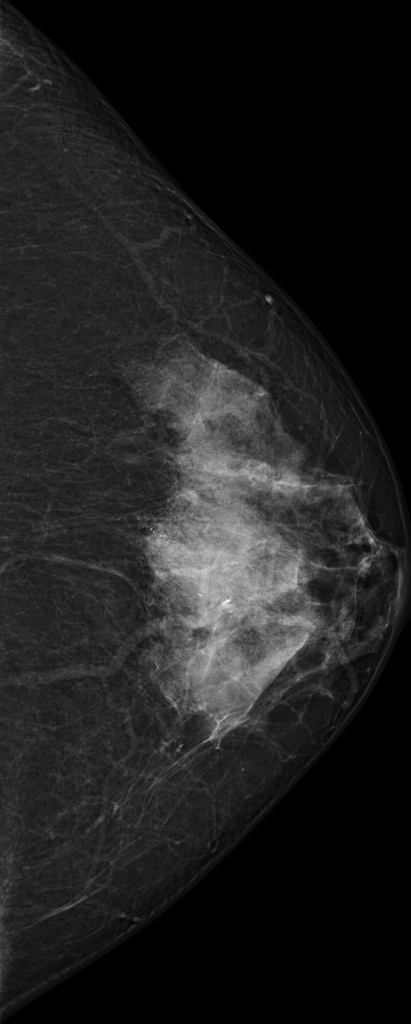
\includegraphics[scale = 0.4]{Final/Figures/Correctly_classify.png}
    % \caption{Well-Predicted Image Sample in classification}
    % \label{fig: classified_True}
    % 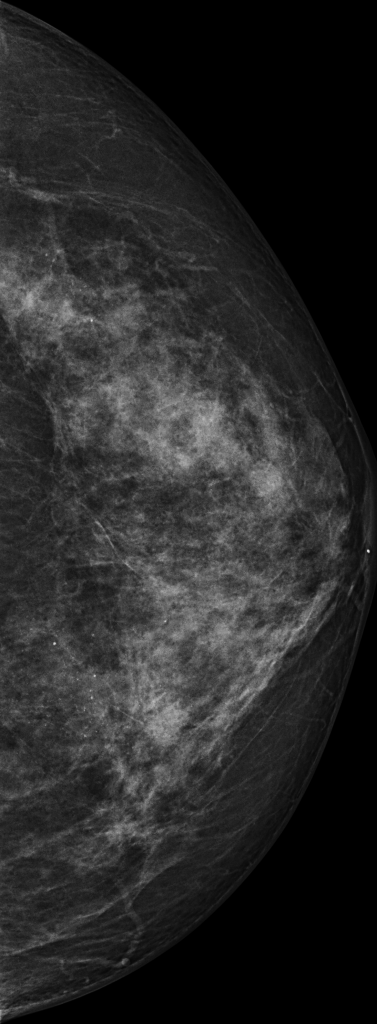
\includegraphics[scale = 0.4]{Final/Figures/Incorrectly_classify.png}
    % \caption{Poorly-Predicted Image Sample in classification}
    % \label{fig: classified_False}
    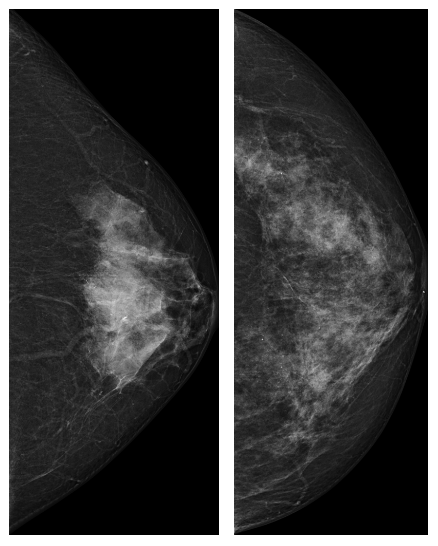
\includegraphics[scale = 0.6]{Final/Figures/predicted_correct:incorrect.png}
    \caption{Well (left) and Poorly-Predicted (right) Image Sample in classification}
    \label{fig: classified_correct+incorrect}    
\end{figure}
%%%%%%%%%%%%%%%%%%%%%%%%%%%%%%%%%%%%%%%%%%%%%%%%%%%%%%%%%%%%%%%%%%%%%%%%%%%%%%%%%%%%%%%%%%%%
\section{Conclusion}
In conclusion, we compared the performance of several models for predicting breast cancer using mammography images and found that our model with the most comprehensive settings outperformed all others. However, we also observed that the dataset was substantially imbalanced in positive cancer cases, with positive cases comprising only 2\% of total images and a count of less than 1,000, which is a very small number compared to its sample size. This likely played a substantial role in the poor test prediction performance. 

The highest-performing Kaggle submission achieved an F1 score of 0.55, which is generally not considered a good performance, but this result partially justified our scores. The difference in the F1 score between the best Kaggle submission model and our model may have been caused by the size of the training data. Specifically, the Kaggle submission used the entire dataset with some external image data, whereas our model used only the data from splitting the dataset into train/test with no additional data to train the model. 

Furthermore, we found that most research in this field uses balanced data with about 10 to 50\% positive case images, which may be a factor in the differences between our results and those of other studies. However, in real-world data, it is more likely to observe fewer patients with cancer out of total observations, which makes our results reasonable given the nature of the data.

Overall, this study presents a meaningful approach for generating good results from imbalanced and small real-world datasets. We tested several models, including CNN and ViT, and found that the researchers' CNN (ResNext) model performed better than all tested ViT models. This was unexpected because ViT models are considered to be well-performed and state-of-the-art models in most other fields using regular image training models, which are similar to our models. Hence, we plan to investigate the hidden reasons behind this behavior and figure out the issue in future studies.

\section{Future Work}
\begin{figure*}[t]
    \centering
    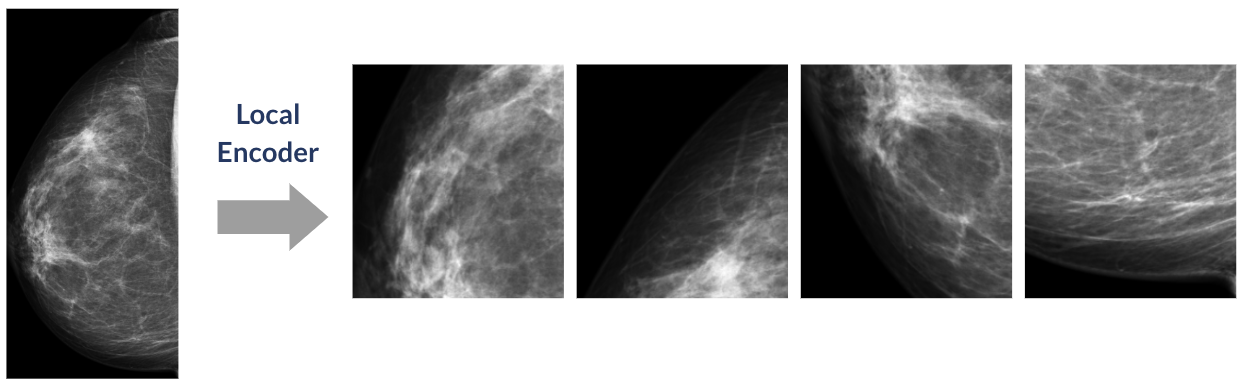
\includegraphics[scale = 0.7]{Final/Figures/future_work.png}
    \caption{YOLOx Image Preprocessing}
\end{figure*}

In this study, we have studied methods to enhance the model and have observed that medical image preprocessing enables a higher prediction accuracy sometimes on simpler models, which is interesting. In future research, we would test some other methods to improve the model's robustness and performance: training ROI extraction (e.g., YOLOx model) on other mammography datasets and a fusion of ROI crop modules that identify optimal centers in the images, thus giving out pixel-level saliency maps and thus identifying better ROI crop patches.

\begin{center}
    \section*{Reference}
\end{center}
{[1]} Wang, H., Zheng, B., Yoon, S. W., & Ko, H. S. (2018). A support vector machine-based ensemble algorithm for breast cancer diagnosis. European Journal of Operational Research, 267(2), 687–699.\\ https://doi.org/10.1016/j.ejor.2017.12.001 \\
{[2]} Vijayarajeswari, R., Parthasarathy, P., Vivekanandan, S., & Basha, A. A. (2019). Classification of Mammogram for early detection of breast cancer using SVM classifier and Hough Transform. Measurement, 146, 800–805. \\https://doi.org/10.1016/j.measurement.2019.05.083\\
{[3]} Karabatak, M. (2015). A new classifier for breast cancer detection based on naive Bayesian. Measurement, 72, 32–36. https://doi.org/10.1016/j.measurement.2015.04.028
{[4]} Pathan, R. K., Alam, F. I., Yasmin, S., Hamd, Z. Y., Aljuaid, H., Khandaker, M. U., & Lau, S. L. (2022). Breast cancer classification by using multi-headed Convolutional Neural Network modeling. Healthcare, 10(12), 2367. \\
https://doi.org/10.3390/healthcare10122367\\
{[5]} Chen, X., Zhang, K., Abdoli, N., Gilley, P. W., Wang, X., Liu, H., Zheng, B., & Qiu, Y. (2022). Transformers improve breast cancer diagnosis from unregistered Multi-View Mammograms. Diagnostics, 12(7), 1549.\\ https://doi.org/10.3390/diagnostics12071549 \\
{[6]} Ragab DA, Sharkas M, Marshall S, Ren J. Breast cancer detection using deep convolutional neural networks and support vector machines. PeerJ. 2019 Jan 28;7:e6201. doi: 10.7717/peerj.6201. PMID: 30713814; PMCID: PMC6354665.\\
{[7]} Tsochatzidis, Lazaros, Lena Costaridou, and Ioannis Pratikakis. 2019. "Deep Learning for Breast Cancer Diagnosis from Mammograms—A Comparative Study" Journal of Imaging 5, no. 3: 37. https://doi.org/10.3390/jimaging5030037\\
{[8]} https://www.kaggle.com/competitions/rsna-breast-cancer-detection/discussion/392449
{[9]} C. Szegedy, W. Liu, Y. Jia, P. Sermanet, S. Reed, D. Anguelov, D. Erhan, V. Vanhoucke, and A. Rabinovich. Going deeper with convolutions. In Proceedings of the IEEE Conference on Computer Vision and Pattern Recognition, pages 1–9, 2015.

%\newpage
%\documentclass[12pt,letterpaper]{article}
\usepackage{graphicx} % Required for inserting images
\usepackage[latin1]{inputenc}
\usepackage{fullpage}
\usepackage{amsmath}
\usepackage{amssymb}
\usepackage{setspace}
\usepackage{hyperref}
\usepackage{float}
\usepackage{fancyhdr}
\usepackage{multirow}
\usepackage[left=0.8in, right=0.8in, top=1in, bottom=1in, headsep=0pt]{geometry}

\begin{document}

\begin{center}
    \subsection*{Appendices}
\end{center}
\begin{center}
    \subsubsection*{Appendix A}
    Model Flow-diagram
\end{center}

\begin{figure}[H]
    \centering
    \hspace{-0.5in}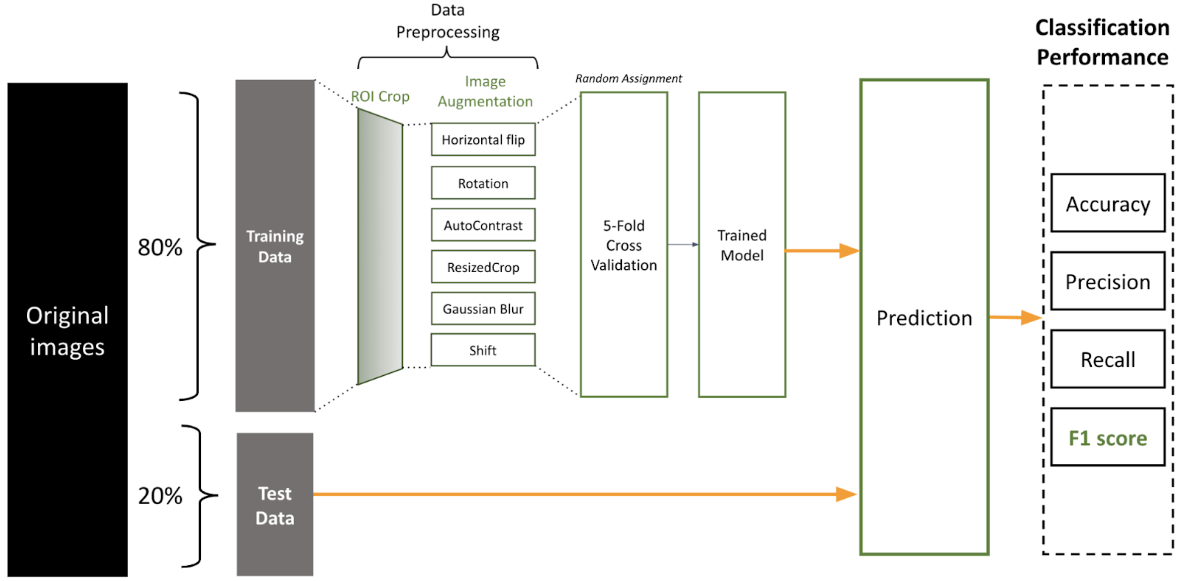
\includegraphics[scale = 0.75]{Final/Figures/model diagram.png}
    % \caption{Model Diagram}
    % \label{fig:final_model_diagram}
\end{figure}

\begin{center}
    \subsubsection*{Appendix B}
    Model Flow-diagram
\end{center}

\end{document}

\end{document}